\section{Search in pure p2p}
In order to find content in a p2p network we can both:
\begin{itemize}
    \item \emph{search}: search in the network based on a set of attributes of the content we are looking for.
    This is similar to google search, it's user friendly because we don't need to build structure over the existing overlay network, but it doesn't scales and adds a huge overhead since we need to compare all the attributes to all the objects in the network;

    \item \emph{addressing}: we can pair a \emph{unique identifier} to the content and use those IDs to retrieve it.
    Usually the ID is the hash of the content (so we have IDs of the same length) and the storage of those associations exploits \emph{Distributed Hash Tables} (DHTs).
    It's main advantage is the efficient object lookup while it's main disadvantage is the management of that addressing structure.
    Moreover this method is not based on location (like URLs) but on content (from which we define the hash of it).
\end{itemize}

\section{DHT}
Distributed Hash Table is a good mid way to optimize both communication overhead and memory needed to address resources:
\begin{itemize}
    \item with $O(N)$ communication overhead and $O(1)$ memory we have the flooding search;
    \item with $O(1)$ communication and $O(N)$ memory we have centralized server;
    \item with $O(log N)$ communication and $O(log N)$ memory we have distributed hash table.
\end{itemize}

Moreover the DHT allows us:
\begin{itemize}
    \item scalability;
    \item avoid false negative because each time we make a search we search in all the network;
    \item the system can self manage both the join of a new node in the system and it's leave, both volunteer leave and faulty one.
\end{itemize}

\subsection{Hashing functions}
In computer science an hash function is a function that maps one piece of data to another fixed-lenght piece of data, which typically is an integer.
Since we are mapping every available input to a fixed-length output we could have collisions.

An hash-table is a key-data store in which the key is hashed directly in order to find a bucket in the hash table, then we insert the value for that key in that bucket.
Each bucket will store values for all the input that colliding produce that bucket index.

In the end a cryptographic hash function must fullfill a set of properties in order to enhance security: mainly low probability of collision.

\subsection{Scaling hash table}
A single hash table of course would be too much to be store on a single peer so we can split the hash table into several parts and distribute it to several servers.

Once we've distributed this table we can use hash of resources to map them to a dynamically changing set of peers in order to access them in a faster way.

\subsection{Rehashing}
If one of the peer, holding a bucket, crashes (or a new peer joins) we have to rebuild the network, this problem is called \emph{rehashing}.
Basically we need to compute part (a large part) of the table in order to accomodate the new number of peers which will result in a lot of data traffic.

\subsection{Consistent hashing}
We can use an hashing scheme that does not depend directly on the number of servers trying to:
\begin{itemize}
    \item minimize the number of keys that needs to be relocated when adding or removing servers;
    \item avoid global reordering of the table.
\end{itemize}

In order to achieve all of those we can use \emph{consistent hashing} which is a hashing technique that guarantees all of the above because:
\begin{itemize}
    \item distribution scheme does not depend directly on the number of servers;
    \item each node manages an interval of consecutive hash keys instead of a set of sparse one;
    \item intervals are splitted/joined when nodes join/leave the network and keys are distributed between adjacent peers. 
\end{itemize}

The key idea is to hash both the resources and the nodes to the same space, this way whenever we are looking for a resource $x$ that hashes to $h(x)$ we can scan the buckets starting from $h(x)$ and going to the right up until we find the first bucket $h(s)$ who has an actual peer whose name $s$ hashes to it. 

In general to build a DHT we have to:
\begin{itemize}
    \item define a common key space for both the nodes and the resources;

    \item we connect the nodes using a small, bounded number of links, such that max hop count is bounded.
    Different connections define different overlay topologies;

    \item define a strategy for assigning items to nodes, using this relation then we can build a search algorithm that exploits this sorting.
\end{itemize}

Let's see a clarifying example: let's assume we want to distribute a set of resources to a set of peers: we first decide to use a logical name space called \emph{identifier space}, which is basically a set of identifiers $\{0, 1, 2, ..., N-1\}$.
We decide that the overlay we want to use is a \emph{logical ring} modulo $N$, to actually build the overlay network we hash the name of the peer (or a random identifier) and wrap it modulo $N$, this way we've mapped the peers to the identifier space we've chosen before.
Successively we define the successor of an identifier as the first node met going in clockwise direction starting at the identifier, now to build the overlay we make each node point to its successor:
\begin{figure}[H]
    \centering
    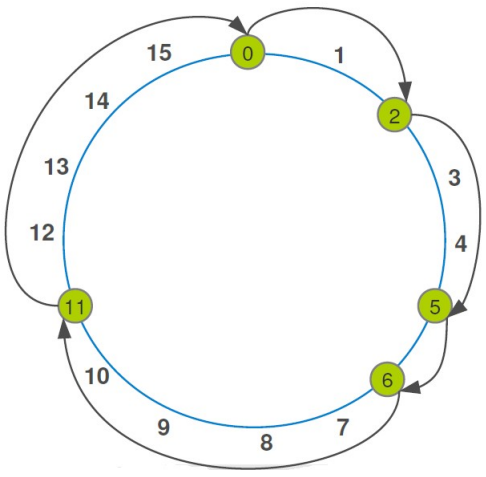
\includegraphics[width=200px]{images/3_DHT/01.png}
    \caption{DHT Overlay}
\end{figure}

To store the resource we use the same technique: we hash the resource and obtain an identifier in the same space, then we store it in it's successor.

If a peer leaves the networks all we have to do is rehash only the resources attached to it, by simply moving them to the successor of the leaving node.

\subsubsection{Properties}
Consistent hashing offers us some interesting properties:
\begin{itemize}
    \item when the hash table changes on the average we only have to move $\frac{k}{n}$ keys ($k$ number of items and $n$ number of servers);
    \item when a node leaves only it's resources must be relocated;
    \item when a node joins we map the keys between the new node and the previous node in the hash ring to point to the new node.
\end{itemize}

Of course the node leave could be:
\begin{itemize}
    \item volunteer: this way the leaving node can advice the neighbours in order to move it's resources to the successor and advertise it's predecessor to update it's successor pointer;
    \item failure: if a node suddenly disconnects from the network all the data it stores are lost if there is no replica so it is important to introduce both data redundancy and information refresh.
    Moreover it is important to probe neighbours for their activity, if a failure happens it is important to update routing table.
\end{itemize}

\subsubsection{Data lookup}
To lookup a key $k$ we need to compute it's hash and follow the successor pointers until item $k$ is found.
This approach is not the most efficient one because in the worst case the lookup is $O(N)$.

To speedup the routing we can set more than one connection, instead of just having a pointer to the successor we can have a pointer to:
\begin{itemize}
    \item $succ(n+1)$;
    \item $succ(n+2)$;
    \item $succ(n+4)$;
    \item ...
    \item $succ(n+2^{M-1})$;
\end{itemize}
this way we can have lookup in $O(log N)$.

The routing table of each node is logarithmic because each node $n$ knows:
$$
    successor(n + 2^{i-1}) for i = 1... M
$$

\subsection{Chord}
The discussed protocol is the base of \emph{CHORD}, developed in 2001 from MIT.

\section{Kademlia}
Kademlia is \emph{the de facto standard searching algorithm for P2P networks on the internet}.
It's a protocol:
\begin{itemize}
    \item \emph{decentralized}: data is stored on a central server, but rather redundantly stored on peers;
    \item \emph{fault tolerant}: if one or more peers drops out of the network, the data, having been stored on multiple peers, should still be retrievable;
    \item \emph{complicated engines are not required}: data stored is key-value pairs so even IoT devices with limited storage can participate in the network.
\end{itemize}

This protocol is used by some of the largest public DHTs:
\begin{itemize}
    \item BitTorrent Mainline DHT;
    \item Ethereum P2P network;
    \item IPFS (Sloppy Kademlia);
    \item KAD network (emule)
\end{itemize}

Some characteristics that Kademlia has:
\begin{itemize}
    \item routing information spreads automatically as a side-effect of lookups: pointers among peers are not symmetric so each node could have some entry in the routing table to use to speedup the research;
    \item flexibility to send multiple requests in parallel to speed up lookups by avoiding timeout delays (parallel routing);
    \item iterative routing: the peer that submits the query is able to control the query at each step, it doesn't use recursive operation called on another nodes.
\end{itemize}

\subsection{Structure of the overlay}
In Kademlia the identifiers of nodes and data are organized in a \emph{complete binary trie}.

The logical identifier space is defined by the leaves of the tree so nodes and content have identifiers in the leaves.
We need a rule to partition the keys (and so the content) among the nodes by respecting the rules of consistent hashing.
Of course not all leaves correspond to nodes, let's take this structure as an example:
\begin{figure}[H]
    \centering
    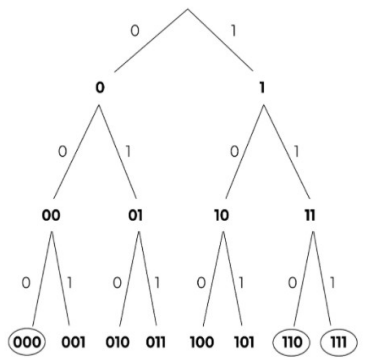
\includegraphics[width=250px]{images/3_DHT/02.png}
    \caption{Circled leaves are nodes}
\end{figure}

A key is assigned to the node with the \emph{lowest common ancestor} which is:
\begin{itemize}
    \item find the longest common prefix between the key and the node identifier
    \item assign the key to that node.
\end{itemize}
With the preceding structure we'd have:
\begin{figure}[H]
    \centering
    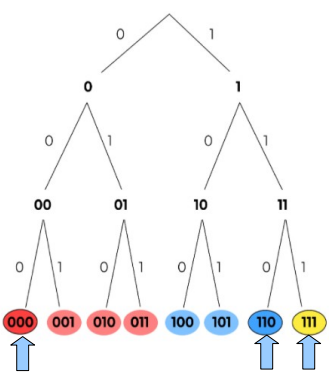
\includegraphics[width=250px]{images/3_DHT/03.png}
    \caption{Structure with association of resources to peers}
\end{figure}

In the case of more peers with the same lowest common ancestor we have an arbitrary situation so we need to improve the notion of closeness in order to break the tie situation and evenly distribute the keys between various tie leaves.

In order to break the tie we:
\begin{itemize}
    \item we look at the most significant bit where they differ, we call that index $b$;
    \item we assign the key to the node whose id bit $b$ equals bit $b$ of the key.
\end{itemize}
for instance in the example we are following we have a tie between 110 and 111 and we have to associate the resources 100 and 101, following the algorithm we'll assign 100 to 110 and 101 to 111.

\subsubsection{Compute closeness (or distance)}
To efficiently compute the distance between a key and a node:
\begin{itemize}
    \item initialize the distance value at 0;
    \item compare the key and computer ID bit by bit;
    \item if the key and the node ID differ at the $i$-th least significant bit, add a penalty of $2^i$ to the distance value.
\end{itemize}
Basically we can compute the xor between the key and the node id taking those values as integers.

In the end a key should be stored on the computer that is closest to the key or has the lowest xor value with the key relative to all other node ids.

\subsubsection{Xor as a metric}
Xor satisfies every properties of a metric:
\begin{itemize}
    \item $d(x,y) = 0$
    \item $d(x,y) > 0 $ if $x \neq y$
    \item $\forall x,y : d(x,y) = d(y,x)$ (symmetry)
\end{itemize}
moreover it satisfies more useful properties:
\begin{itemize}
    \item $d(x,y) \bigoplus d(y,z) = d(x,z)$ (transitivity)
    \item $d(x,y) \bigoplus d(y,z) \geq d(x,z)$ (triangular inequality)
    \item given $x$ and a distance $\Delta$, it exists a single $y$ such that $d(x,y) = \Delta$ (unidirectionality)
\end{itemize}

Symmetricity enables Kademlia to learn contacts from ordinary queries it receives, this helps in building the routing tables.

Unidirectionality instead tells us that there is a single node at minimal distance with the key so lookups for the same key will converge to the same path, since this is true we can cache tems along the path in order to avoid hotspots.

Moreover the metric is related to the identifier prefix so the larger the common prefix, the smaller the distance.

It is important to notice that according to the xor metric, the key is closer to any node in its subtree than nodes in other subtrees, for example: 1000 and 0111 despite being literally one after the other have a distance of 15.
Let0s consider two identifiers $x$ and $y$ of length $L$ that share a common prefix of length $p$ and differ in the last $i=L-p$ bits, then their distance, according to xor metric will be such that:
$$
    2^{i-1} \leq d(x,y) < 2^i
$$
those bounds enables to pair the nodes of the subtree with an identifier range.

\subsubsection{Peers tree}
Of course the peers in the network are much lesser than the identifiers because the space of identifiers is huge nd not all the identifiers are paired with a peer.
The peer tree is an unbalanced binary tree showing only the identifiers of peers present in the network so we have a leaf for each peer, not for every identifier.

In this way we can compress the tree using only the used prefixes because the prefix uniquely identifies the peer.

\subsection{Routing}
The goal of the routing in the overlay network is to define a look-up procedure in order to find a key (and it's associated resource) storing only the addresses of a small amount of nodes, in a quick way.
Moreover we would like to get us at least one bit closer to the key at each query step bringing the runtime to $O(log N)$.

The main idea is to store just a logarithmic number of node ids and their corresponding IP addresses and then some contact taken from the identifier trie.
To achieve that we can start from the node identifier and take the path from that node to the root: for every sibling node of a node met on the path we:
\begin{itemize}
    \item store the identifiers of $k$ nodes whose ids are descendant of the sibling;
    \item each \emph{sibling bucket} contains $k$ contacts for each level, we call it a $k$-bucket.
\end{itemize}

Each row of the routing table obtained contains a $k$-bucket, so $k$ contacts.
Each row corresponds to a subtree and each contact stores (ID, IP, UDP port).
Row $i$ contains contacts with distance $d$ such that $2^{i-1} \leq d < 2^i$ and each entry corresponds a common prefix: the lower the entries the longest the common prefix.
Nodes in each bucket are maintained ordered such that least recently contacted nodes are in the first positions of the list.

\subsubsection{Add contact}
\begin{figure}[H]
    \centering
    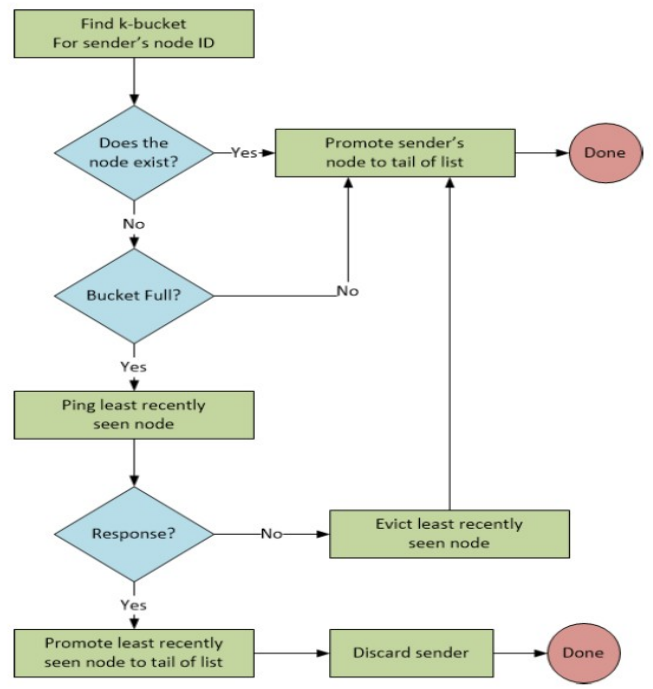
\includegraphics[width=250px]{images/3_DHT/04.png}
    \caption{Algorithm to add contact to the routing table}
\end{figure}

The protocol prefers older contacts with respect to newer ones because, as shown in Gnutella collected trace: the longer a node has been up, the more likely it is to remain up another hour, so by keeping the oldest live contacts around, $k$-buckets maximize the probability that the nodes they contain will remain online.
Moreover this strategy empowers the resistance to certain DoS attacks because an attacker now can't flush the nodes routing state by flooding the system with new nodes.

\subsubsection{K-bucket periodic refreshment}
The add contact policy allows continuous update of the $k$-bucket list, however it may be the case that a $k$-bucket is not refreshed for a given period of time due to the lack of messages from nodes in the range covered by that bucket.
In order to fix this case a refresh is periodically executed (once each hour):
\begin{itemize}
    \item Kademlia chooses an identifier belonging to the range covered by the bucket at random and search that identifier;
    \item if the node with that identifier sends a reply it is inserted in the $k$-bucket
\end{itemize}

\subsection{Key look-up}
In order to make a key lookup we find the closest node to the key in the routing table, of course via xor distance.
If that node does not have the key and has not already responded, we ask it for the key of a closer node, if otherwise it responds then we update our closest nodes set.

The goal of each iteration is to reduce by $\frac{1}{2}$ the xor distance and update to a smaller size $k$-buckets.

At each step we can propagate the query to more than one node in that $k$-bucket, let's call this number $\alpha$.
Let's see an example of lookup in the case of $\alpha = 1$:
\begin{figure}[H]
    \centering
    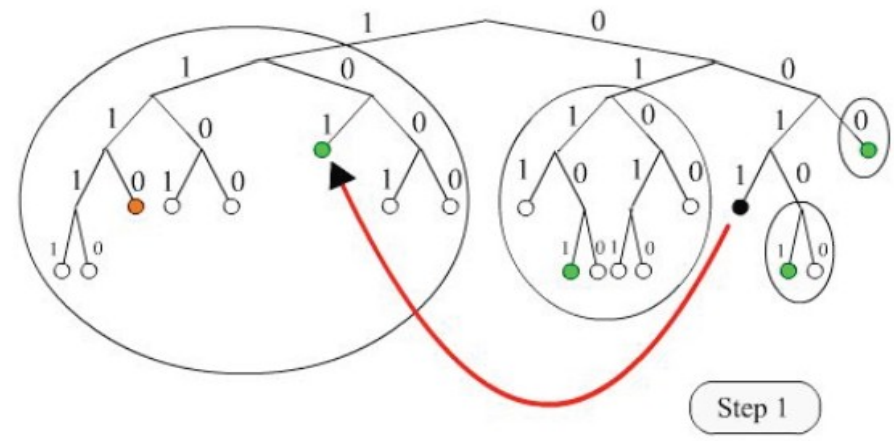
\includegraphics[width=250px]{images/3_DHT/05.png}
    \caption{Lookup: step 1}
\end{figure}
We start from black node (0011), and we want to query the orange node (1110), we compute the nearest node via our routing table which contains some bucket (green node are the buckets content).
We query the green node in the image and it tells us that it doesn't know were the target is, but gives us the information about it's nearest peer:
\begin{figure}[H]
    \centering
    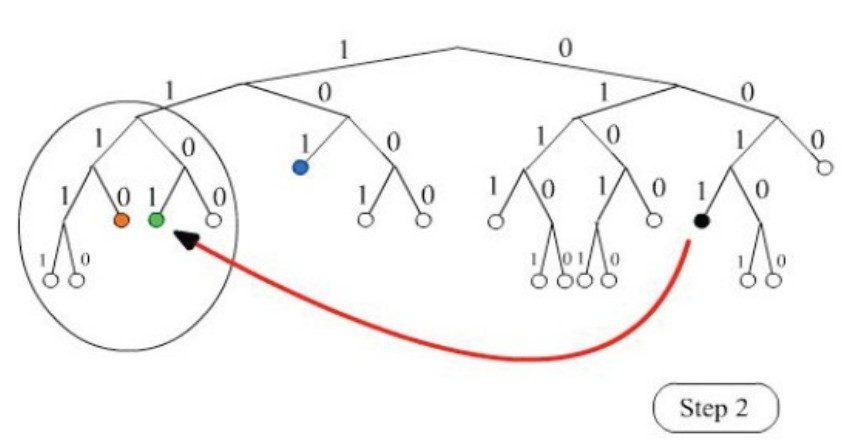
\includegraphics[width=250px]{images/3_DHT/06.png}
    \caption{Lookup: step 2}
\end{figure}
Then we query the previous resulted peer and so on and so forth until we reach the subtree we are looking for and find out the actual target node.

As we can see at each step the prefix match increases of at least one bit: we have $O(log N)$ search.

NB: the shown one is called \emph{iterative} routing because at each step is still the same node to perform the query to the other nodes, however there exists the \emph{recursive} routing in which each queried node perpetuates the next step of the query and in the end the response gets back propagated to the original issuer.
Kademlia uses iterative routing because despite producing more traffic the original node has a way to update it's internal routing table.

\subsubsection{Parallel routing}
In order to speed up the lookup process we can query different peers with different distance from the target, this way the probability of  hitting a node who directly know the target of our query is much greater.

\subsubsection{Remark}
The dispatch of the query to the node which is closest to the target not necessarily implies the smaller path toward the target, however the unidirectionality of the xor metric guarantees that all the paths converge toward the target.
In order to speedup the search the query is sent to the $\alpha > 1$ nodes closest to the target.

\subsection{Basic protocol operations}
Kademlia protocol consists of 4 primitive operations defined as \emph{Remote Procedure Calls} exploiting UDP connections.

\subsubsection{Find node}
\begin{verbatim}
    FIND_NODE v->w (T) (v, w nodes, T target of the lookup)
\end{verbatim}
The node $w$ returns $k$ triples (IP address, UDP port, Node ID) for the $k$ nodes closest to the target $T$ that it knows.
Those triples can come from a single $k$-bucket or from multiple ones if the closest $k$-bucket is not full.

\subsubsection{Find value}
\begin{verbatim}
    FIND_VALUE v->w (T) (v, w nodes, T value looked up)
\end{verbatim}
It is used to lookup for a value and not a node, the input $T$ is a 160 bit ID that represent a value, if the corresponding value is present in the queried node $w$ the associated data is returned, otherwise the node returns a triple, behaving as a \verb|FIND_NODE| primitive.
In that second case it is issuer job to return continue searching for the desired value.

\subsubsection{Ping}
\begin{verbatim}
    PING v->w
\end{verbatim}
Used to probe node $w$ to see if it is online.

\subsubsection{Store}
\begin{verbatim}
    STORE v->w (key, value)
\end{verbatim}
Used to instructs a node $w$ to store a key-value pair.

\subsubsection{Full algorithm}
\begin{figure}[H]
    \centering
    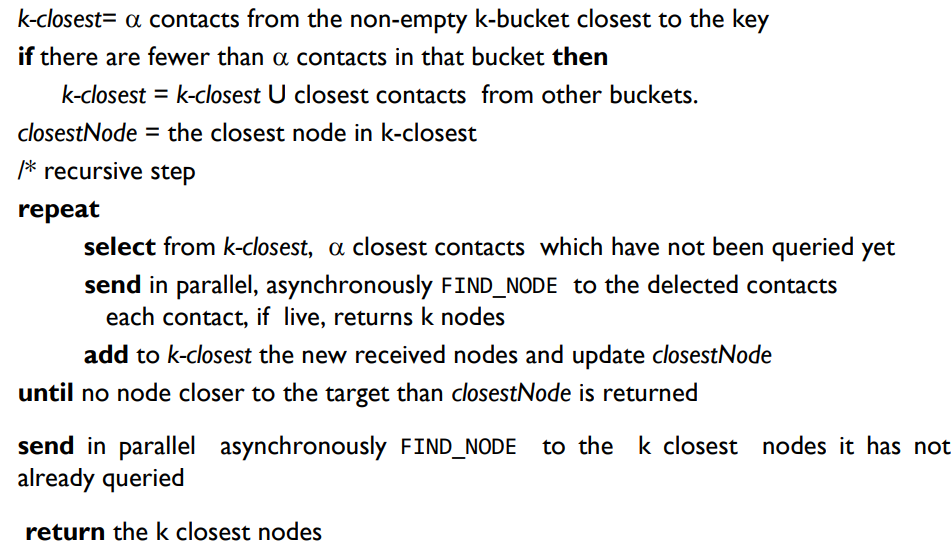
\includegraphics[width=300px]{images/3_DHT/07.png}
    \caption{Full search algorithm}
\end{figure}

\subsection{Storing values}
To store a key-value pair the publisher node performs a look-up to find the $k$ closest node to the key and sends them the \verb|STORE| RPCs, so data is replicated on those nodes.

In order to keep values alive in the network there are some \emph{re-publishing} mechanisms, basically each node re-publishes his pairs as necessary to keep them alive when:
\begin{itemize}
    \item some of the $k$ nodes that initially got the key-pair leave the network;
    \item new nodes enters the network with an identifier closer to the key than the nodes on which the key-value pair was originally published.
\end{itemize}

More specifically for file sharing application based on Kademlia the original publisher of a key-value pair is required to republish it every 24 hours.

\subsection{Node join}
When a \emph{new} node joins the network it borrows an alive node's ID which is offline.
The initial routing table of the new node has a single k-bucket containing itself and a \emph{boot} node, then this new node sends \verb|FIND_NODE(new)| to the boot node in order to learn about other nodes which are near to itself, this way some high index k-buckets are filled.

After this set of queries other nodes start to know the new one and insert it in their routing tables.
In the end the new node performs \verb|FIND_NODE(ID)| with an ID further away than its own k-bucket generated at random, this way all the other k-buckets are enriched with more information.

\subsection{Maintenance}
The refresh of k-buckets for which there was no contact within a certain time (like an hour) is done by looking up random ID in a  bucket.

\subsection{Storage \& Caching}
To store a value it's needed to locate the $k$ closest nodes to the ID via lookup, then store the value on those nodes.
Values are considered \emph{soft-state} so they need to be refreshed, moreover values are cached at the first node on a path that did not knew it.

\subsubsection{Node leave}
The node leave does not require much operations, simply if it does not reply, then it will be discarded from the k-buckets.

\subsection{Chord vs Kademlia}
Kademlia defines a flexible routing table with symmetric distances and various alternative paths.
Moreover it's routing table management has a lower cost and the round trip time of the queries can be stored in order to choose the contact with lower RTT during the next lookup.
In the end the symmetricity enables each node to enrich its routing table through the query, while in Chord this is not possible because if a node $x$ receives a query from node $y$ it could be possible that $x$ may not have a pointer to $y$, so the information in the query cannot be generally exploited to enrich the finger table.

\section{Prefix matching DHT}
Kademlia is an instance of the more general concept of prefix-matching DHT.
The prefix routing (or plaxton routing) is a mechanism for the efficient diffusion of object over a network and was published in 1997, before p2p systems came out.

The basic idea is to generalize the routing on hypercubes: we map nodes and keys to a numbers of $m$ digits of a certain base, then assign each key to a node with which it shared the longest prefix if possible.

Some other algorithms of this family are Pastry and Tapestry.

\section{BitTorrent}
The main idea behind BitTorrent is to build a p2p CDN (Content Distribution Network), so a way to spare content around a network.
It starts from a single server who exposes that content and then it is copied in more peers, moreover in BitTorrent the content is not fully copied at once, rather split in chunk and then those chunk are spread in the network in order to increase it's presence in the network.

Moreover BitTorrent does not implement all the functions of a typical p2p system, for example searching is not implemented, rather it is meant to be fully integrated with the web.
Basically there exists several web server whose job is to share file descriptors that than can be used to search for peers who expose chunks of that file.

BitTorrent also implements file swarming which means that a peer makes whatever portion of the file that is downloaded immediately available for sharing.

\subsection{Tracker}
A tracker is a node that take trace of peers who are currently providing the content.
This way whoever wants to download the content just has to query the tracker in order to know information to directly connect to the other peers.
Once the transfer of that chunk is completed, then the peer announces to the tracker that now it can provide the content too.

\subsection{Glossary}
\begin{itemize}
    \item the file with extension \verb|.torrent| is a descriptor of the file to be published on a server.
    It contains reference to a tracker and information on every chunk of the file to be published;

    \item swarm: is the set of peers collaborating to the distribution of the same file coordinated by the same tracker;

    \item seeder: is a peer which owns all the parts of the file.
    At the beginning there is only one seeder, once the content is completely shared with some other peers, then they can become seeder too if continue to expose the file.
    Some algorithms are used in order to push rarest file chunks in order to improve the distribution across the network.

    \item leecher: is a peer which has some part or no part of the file and downloads the file from the seeder and or from other leechers.
\end{itemize}

\subsection{Blocks}
Content is split into chunks called \emph{pieces} (256KB to 2MB), she SHA-1 of each piece is stored in the .torrent file.
Once a peer receives a piece it becomes the seed of that piece.

Pieces however are split into \emph{blocks} or \emph{subpieces} of 16KB, this is done because BitTorrent uses TCP connections.
In order to fool the slow start mechanism of TCP and avoid that the connection gets capped to a slow rate we split in subpieces in order to have always something to transmit on those connections.
The protocol always tries to have some number of requests for a sub-piece pipelined at any time.

\subsection{Pieces selection algorithms}
If an inefficient policy is used to pick pieces to transmit peers may end up in a situation where each peer has all identical set of easily available pieces and none of the missing ones.

\subsubsection{Strict priority}
If a subpiece of a piece has been required, all the other subpieces of the same piece are required before requiring another block.

The goal of this algorithm is the fast assemblage of the pieces because only the complete of pieces may be exchanged with other peers.
Moreover each peer tries to assemble in the fastest way complete pieces.
In the end the chocking algorithm favour the peers which have entire pieces to exchange with the partners.

\subsubsection{Rarest first}
Each peer knows the pieces owned by the others so it can have a local view of the availability of each piece.
This algorithm selects a piece among the rarest set.

\subsubsection{Random first piece}
Initially a leecher does not own any piece and cannot offer anything to the other peers of the swarm, since it is important that a peer acquires a piece as soon as possible the rarest first policy cannot be used.
To solve this problem the first 4 pieces are downloaded through the random first piece policy.
It is also known as \emph{fast starting}, then after that the rarest first policy is used.

\subsubsection{Endgame}
Most downloads slow down when approaching the end of the download because peers characterized by low bandwidth slows down when transfer is going to end and the download from those peers cannot be overlapped to the download from other peers.

The endgame policy specify that the last pieces of the file to download are required to all the peers that own the file.
To avoid bandwidth waste when the piece is received from the peer which has requested it the download started in parallel are cancelled, this is a small waste of bandwidth since the end game is executed for a small period of time.

\subsection{Choose the peers}
In choosing the peers to talk with we have to keep in mind the problem of free riders.
A free rider is an individual who doesn't pay its price and gives to others the burden to pay the good.

In BitTorrent a free rider is a peer that doesn't put his bandwidth at disposal of the community.
The resolution of this problem is complex because:
\begin{itemize}
    \item no centralized entity may control the nodes exists;
    \item it is not possible to impose a given behavior to the BitTorrent clients because everyone can implement it's client version;
    \item a solution exploiting dynamic monitoring is needed.
\end{itemize}

The behavior of the whole BitTorrent network depends on the \emph{cooperative behavior} of the peers with respect to the community, so it is important to remove or limit the free riders.
A possible approach is based on \emph{reciprocity}: a client obtains a good service if and only if it gives a good service to the community.
This policy forces the egoist peers to have a good behavior, moreover it's based on connection monitoring and has been developed around the \emph{tit for tat} strategy from game theory (result of the iterated prisoner dilemma problem).
The implementation in BitTorrent is the choking/unchoking algorithm.

\subsubsection{Chocking algorithm}
The idea is to chock the connection: a temporary refusal to upload to another peer but maintaing the possibility to download from it.
The principle is to upload to peers who have uploaded to us.

Each peer periodically:
\begin{itemize}
    \item evaluates, for each neighbour, the download speed in the previous round and decides which neighbour it is going to choke;
    \item unchok a fixed number of peers, 4 by default.
\end{itemize}
The decision on which peers to unchok is taken every 10 seconds by each peer and it is based on the download rate on the last $X$ seconds to avoid the TCP slow-start rapid choking and unchoking to fake the metrics.

We can summarize in: if our upload rate is high more peers will allow us to download from them, as a reward we can get a higher rate in download from the neighbours.

\subsection{Connection status}
Each peer maintains for each remote peer it is connected the following flags:
\begin{itemize}
    \item \verb|am_chocking|: true if we are chocking the connection with the other peer;
    \item \verb|am_interested|: true if we are interested in at least a piece on the remote peer;
    \item \verb|peer_chocking|: true if the remote peer is chocking connection with us;
    \item \verb|peer_interested|: true if the remote peer is interested in at least one piece we own
\end{itemize}
We can receive data from a remote if the local peer is interested in the remote per and the remote peer unchocked the connection to us.

\subsubsection{Optimistic unchocking}
Policy used to avoid to ignore peers that recently join the network and that would be chocked by the previous rules.
Every 3 rounds (30 seconds) an interested and chocked peer is selected at random to be optimistic unchocked, then if this connection turns out to be better than one of the existing unchcked, then it will replace it.
This policy will allow newcomers to download resources and grow.

\subsubsection{Anti snubbing}
When over a minute has gone by without receiving a single sub-piece from a particular peer, do not upload to it except as an optimistic unchocke.

Moreover if chocked by everyone, increase the number of simultaneous optimistic unchocke to more than one.

\subsubsection{Upload only}
In the case we completed our download and now we are only uploading to others the previous algorithm is discarded.
Instead we unchoke peers with the highest upload rate ensuring that pieces get uploaded faster and so replicated faster.

\subsection{Two way handshake}
Once a TCP connection is enstablished with one of the peer received by the tracker a client perform a two-way handshake using the following packet:
\begin{figure}[H]
    \centering
    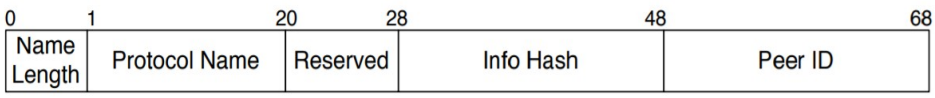
\includegraphics[width=200px]{images/3_DHT/08.png}
    \caption{Two-way handshake packet}
\end{figure}
with the fields:
\begin{itemize}
    \item name length set to 0x13;
    \item protocol name set to \verb|BitTorrent protocol|;
    \item reserved: used to signal extensions to the basic protocol;
    \item SHA-1 hash of the torrent's file infohash;
    \item peerID: the client random ID.
\end{itemize}
Who receives the TCP connection can check the info hash and refuse the connection if the hash does not correspond to any hash of the files it is participating to download.

\subsection{Peer wire protocol}
First message sent after the handshake by both the peers is a bitfield which succintly describes the pieces that the peer has (it's basically a bloom filter).

Then the leecher sends a packet specifying in which index it is interested and the seeder responses with chocke/unchocke notifing wether the download request has been accepted or not.

Once the peer is unchocked it exploits the piece choosing algorithm to decide from which piece to start and notifies it to the seeder via the triple (index, begin, length).
This request can only be sent after being unchocked from the seeder.

Then the seeder responds with the piece (index, begin, block) in which the index is the subpiece \verb|index| in the piece, that starts with an offset \verb|begin| and then the \verb|block| is the actual data.

There is one more packet which is the \verb|Have| packet sent from a leecher to the other peers in order to update other peers that now it holds the new piece.
This packet is useful to monitor swarm because we can understand who has what.

Then there is the packet \verb|Not interested| used to specify that a leecher is not anymore interested in that piece.
It can be sent after receiving a \verb|Have| packet.

The message \verb|Cancel| is sent from a peer to another to indicate that it already got a piece and it is not interested in it anymore.
It is used in endgame mode only.

\subsection{BitTorrent Mainline DHT}
In BitTorrent we still have a centralized server that performs the tracking, but this part requires very little resources compared to distributing the files but can still be a bottleneck and target of several attacks.
BitTorrent Mainline DHT decentralizes the tracker services.

Kademlia is used to implement the DHT instead of a single tracker.
Each node of the DHT stores a part of the tracker information so now each peer implements both BitTorrent wire protocol, for data transmission (over TCP) and a DHT protocol for tracker data transmission (over UDP).

Some of the protocol messages that are implemented are:
\begin{itemize}
    \item \verb|PING|: probe a node's availability or announce one's existence.
    If the node fails to respond for some period of time, it will be purged out of the routing table;

    \item \verb|GET_PEERS(H)|: look for peers belonging to the swarm for the content with infohash $H$.
    The contacted node may store peers for $H$ and so reply with a \verb|PEER| message containing them, or have no info for $H$ and so responding with the identifiers of the 8 peers closest to $H$;

    \item \verb|ANNOUNCE_PEER|: a peer announces it belongs to a swarm;

    \item \verb|FIND_PEER(target_id)|: request for nodes which are clos to the node with node ID \verb|target_id|.
\end{itemize}


